
\documentclass[10pt]{article}


% Define margins
\setlength{\topmargin}{-1.0cm}
\setlength{\oddsidemargin}{0.1cm}
\setlength{\textwidth}{16.5cm}
\setlength{\textheight}{23.0cm}
\usepackage{booktabs} % For prettier tables
\usepackage{placeins}
\usepackage{subcaption}

\usepackage{amsmath}
\usepackage{graphicx} %LaTeX package to import graphics
\usepackage{listings}
\graphicspath{{images/}} %configuring the graphicx package
\usepackage{caption}

\usepackage{xcolor}
\definecolor{blue}{RGB}{0,0,255}
\definecolor{red}{RGB}{255,0,0}
\definecolor{gray2}{RGB}{128,128,128}
\definecolor{gray3}{RGB}{192,192,192}
\definecolor{darkgreen}{RGB}{0, 128, 0}
\definecolor{trq}{RGB}{90, 200, 160}
\renewcommand{\lstlistingname}{}

\lstdefinestyle{cppstyle}{
  language=C++,
  basicstyle=\small\ttfamily,
  keywordstyle=\color{blue}, % Default style for standard keywords
  commentstyle=\color{green!40!black},
  stringstyle=\color{red},
  numberstyle=\tiny\color{gray},
  basicstyle=\ttfamily\footnotesize,
  breaklines=true,
  captionpos=b,
  keepspaces=true,
  numbers=left,
  showspaces=false,
  showstringspaces=false,
  showtabs=false,
  tabsize=2,
  frame=single,
  frameround=tttt,
  framesep=5pt,
  rulecolor=\color{gray},
  breaklines=true,
  captionpos=b,
  showstringspaces=false,
  morekeywords={threadIdx, blockDim, blockIdx, __global__, __device__, __shared__},
  emph={[1]__syncthreads,[2]atomicAdd}, % Add atomicAdd to the emphasized list
  emphstyle={[1]\color{trq}}, % Style for __syncthreads
  emphstyle={[2]\color{magenta}}, % Unique style for atomicAdd
}


% Define header and footer
\usepackage{fancyhdr}
\pagestyle{fancy}
\fancyhf{}
\lhead{{
\includegraphics[height=.70cm]{images/Uni-ljubljana.png}}}
\rhead{\textbf{\textit{Final Project Report for PDSA}} }
\cfoot{\textbf{\textit{\thepage}}}
% \lfoot{\textbf{\textit{Page \thepage/\pageref*{LastPage}}}}
% \rfoot{\textbf{\textit{Alejandro Romero Prieto}}}
% \renewcommand{\footrulewidth}{0.7pt}
\renewcommand{\headrulewidth}{0.7pt}
\setlength{\headheight}{23pt}

% This is to define a style with no footer for the table of contents
\fancypagestyle{nofooter}{%
  \fancyfoot{}%
}

% To manage references
\usepackage{natbib}

\begin{document}

% Title Page %%%%%%%%%%%%%%%%%%%%%%%%%%%%%%%%%%%%%%%%%%%%%%%%%%%%%%%%%%%%%%%%%%%%%%%%%%%%%%%% 

\begin{center}
% \vspace*{\baselineskip} % Original - You can reduce or remove this line to move content up
\vspace*{-1cm} % This moves the content up by 1 centimeter



\includegraphics[width=0.5\textwidth]{images/University-of-Ljubljana.png}\\
\vspace*{2cm}

{\huge \textbf{Histogram Equalization with Cuda}}

\vspace*{3\baselineskip}

{\LARGE \textbf{Final Project Report for Class: \\ Parallel and Distributed Systems and Algorithms }}

\begin{large}
\vspace*{2\baselineskip}

Date: 05/02/2024

\vspace*{4\baselineskip}

\emph{by Undergraduate Student} \\[1ex]
%Submitted by \\[\baselineskip]
{\Large Irinej Slapal \\ \par} % Editor list
{{ 63200268}}\\[2cm] % Editor affiliation


\emph {Under the supervision of} \\ % Tagline(s) or further description
[\baselineskip] % Tagline(s) or further description
{\Large Prof. Dr. Patricio Bulić\\ \par}

\vspace*{4.5cm}

% 	{\scshape  \today} \\[0.3\baselineskip] % Year published
{University of Ljubljana}\\
{\large Faculty of Computer and Information Science}\par % Publisher

\thispagestyle{empty} 

\end{large}
\end{center}
\pagebreak


% Contents %%%%%%%%%%%%%%%%%%%%%%%%%%%%%%%%%%%%%%%%%%%%%%%%%%%%%%%%%%%%%%%%%%%%%%%%%%%%%%%%%%%%%%%%

% \lhead{\emph{Contents}} % Set the left side page header to "Contents"
\tableofcontents
	\thispagestyle{nofooter}
	%\include{abstract/abstract}
	\cleardoublepage
	\typeout{}

\pagebreak
% Main Content %%%%%%%%%%%%%%%%%%%%%%%%%%%%%%%%%%%%%%%%%%%%%%%%%%%%%%%%%%%%%%%%%%%%%%%%%%%%%%%%%%%%
\setcounter{page}{1}

\section{Introduction}
\label{sec:Introduction}
% Introduction content goes here.
 Histogram equalization is a fundamental technique in the field of digital image processing, used for improving the contrast of images. The primary goal of this method is to adjust the intensity distribution of an image, so that it spans the entire range of possible values more uniformly, so that the probabilities of all gray levels are somewhat close to equal. 
\\ Many images, especially those captured in low-light conditions or with limited dynamic range sensors, have poor contrast, resulting in concentration of pixel values in a narrow intensity range. This method is particularly useful for such images, adding contrast and bringing in details, invisible beforehand, to ones attention. \\
The process of calculating a histogram is reading a color level (in this case, 8-bit grayscale level) from each pixel and track the appearance for each value. Finally the histogram shows how many pixels have a certain gray scale value.  
\\
The histogram $H$, we get from image, is the length of $L$:
\\
\\
\begin{equation*}
    H = \{n_0, n_1, n_2, \ldots, n_{(L - 1)}\}
\end{equation*}
\\
Each value in histogram is equivalent to the number of pixels with the gray scale value $l$,\\ $l \in [n_0, n_{L-1}]$. The probability of pixel having gray scale value of $l$, in an image, the size of $N \times M$ is calculated as:
\begin{equation*}
    p(l) = \frac{n_l}{N \times M}
\end{equation*}
\\
The normalized histogram then contains the probabilities of the appearance of the different grey levels

\begin{equation*}
    H_{\text{norm}} = \{p(0), p(1), p(2), \ldots, p(L - 1)\}
\end{equation*}
\\
The cumulative distribution function tells us if $X \le x$.\\
CDF corresponding to $n_l$ is:
\begin{equation*}
    cdf(l) = p(X < l) = \sum_{i=0}^{l} p(i)
\end{equation*}


\begin{figure}[ht]
  \centering
  % Subfigure for the original histogram
  \begin{subfigure}[b]{0.4\textwidth}
    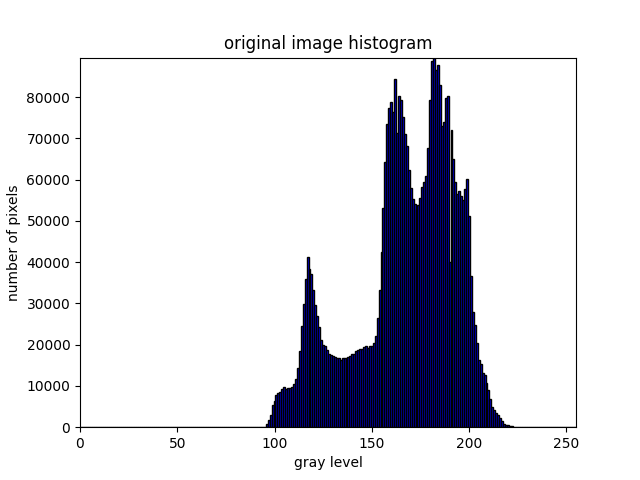
\includegraphics[width=\textwidth]{images/buca-h.png}
    \caption{Original image histogram}
    \label{fig:original-histogram}
  \end{subfigure}
  % Subfigure for the equalized histogram
  \begin{subfigure}[b]{0.4\textwidth}
    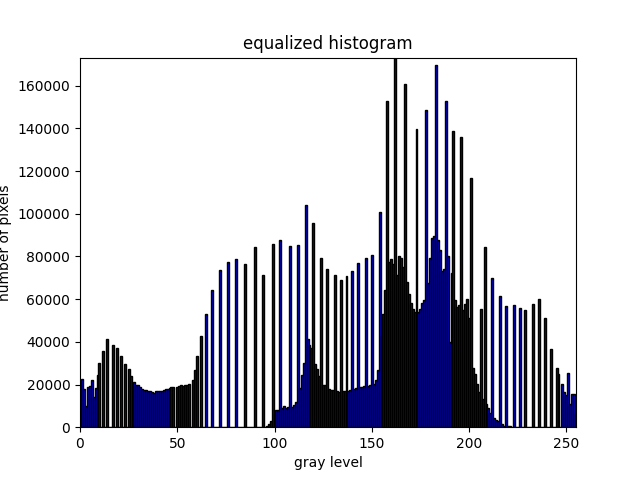
\includegraphics[width=\textwidth]{images/buca-e.png}
    \caption{Equalized histogram}
    \label{fig:equalized-histogram}
  \end{subfigure}
  \caption{Comparison of original and equalized histograms, for image buca1.jpg}
\end{figure}


\emph{To sum it up:} Histogram equalization redistributes the intensity values of an image, thereby enhancing its overall contrast and making details more visible. 

\pagebreak

\section{Parallel implementation with Cuda}
\vspace{0.5cm}
% Details on how to calculate histogram.
\subsection{Histogram Calculation}
\vspace{0.3cm}

Bellow is a sequential function for calculating Histogram from an image in C programming language.
Notice, that the function iterates through every pixel in given image. 
\begin{lstlisting}[style=cppstyle]
void CalculateHistogram(unsigned char* image, int width, int height, unsigned int *histogram){
    //Calculate histogram
    for (int y=0; y<height; y++) {
        for (int x=0; x<width; x++) {
            histogram[image[y*width + x]]++;
        }
    }
}
\end{lstlisting}

There often is a case of image being too large, where the sequential approach would take too long.\\

There is a faster approach, in which threads are used to compute the histogram in parallel, as shown bellow:

\begin{lstlisting}[style=cppstyle]
__global__ void CalculateHistogramKernel(unsigned char* image, int width, int height, unsigned int *histogram){
   
    // calculate global x, y of pixel on image
    int x = blockIdx.x * blockDim.x + threadIdx.x;
    int y = blockIdx.y * blockDim.y + threadIdx.y;

    // calculate local x, y of pixel in block 
    int lx = threadIdx.x;
    int ly = threadIdx.y;

    // allocate local memory for local histogram for each block
    __shared__ unsigned long localHistogram[GRAYLEVELS];

    // each thread sets its pixel in local (block) histogram to 0 
    localHistogram[blockDim.x * ly + lx] = 0;
    __syncthreads();

    //read value from image and increment local histogram according to its GRAYLEVEL
    if (x < width && y < height) {
        atomicAdd(&(localHistogram[image[y * width + x]]), 1);
    }
    __syncthreads();

    //Finnaly coresponding local threads from each block sum their vaues to form a complete histogram
    atomicAdd(&(histogram[ly * blockDim.x + lx]), localHistogram[ly * blockDim.x + lx]);
}
\end{lstlisting}

\vspace{1cm}

This kernel assigns each thread a unique pixel in the image, using the thread's global X and Y coordinates calculated from CUDA's built-in blockIdx, blockDim, and threadIdx variables.
BlockSize must be 256 (16*16) here, so that histogram (which has length of 256) is correctly calculated.\\  
GridSize is then calculated according to the size of input image, so that blocks "cover" the whole image.\\
To optimize memory usage and access speed, shared memory is used within each block to store a local histogram of pixel intensities for each block in the grid.\\

\pagebreak

Threads within a block read their corresponding pixel's intensity from the image stored in global memory and increment the appropriate entry in the local histogram.\\
Atomic operations are used, to avoid race conditions. After synchronizing all threads within the block to ensure the local histogram is complete, each thread then contributes its portion of the local histogram to a global histogram stored in global memory.\\
This approach utilizes the fast shared memory for intermediate calculations and optimizes global memory access. 

\vspace{0.5cm}

\subsection{Comulative Distribution Function (CDF) Calculation}
% Details on calculating the Cumulative Distribution Function (CDF).
\vspace{0.3cm}

The Cumulative Distribution Function (CDF) is a statistical measure used to describe the distribution of a random variable. \\
In the context of image processing and analysis, the CDF of an image's pixel intensities provides a cumulative sum of the histogram counts, up to a certain intensity level. Essentially, for any given intensity value, the CDF indicates the proportion of pixels in the image that have an intensity less than or equal to that value. \\

\begin{figure}[h]
\centering
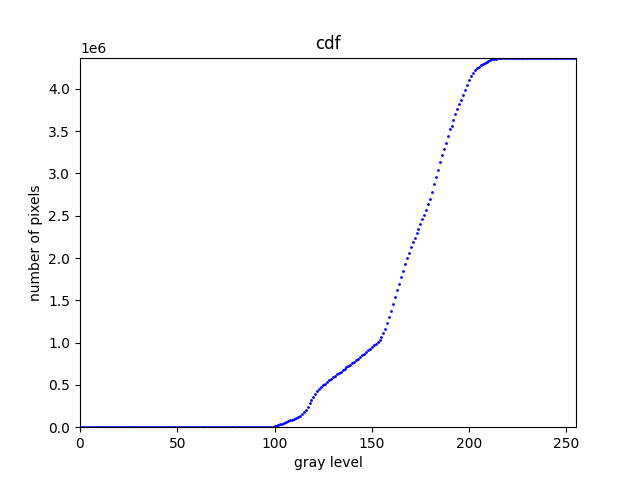
\includegraphics[width=0.5\textwidth]{images/buca-c.png}
\caption{Comulative distribution function for image buca1.jpg.}
\label{fig:mbk}
\end{figure}

\vspace{1cm}

In order to cumulatively sum histograms values (each value in resulting histogram, being the sum of all of its previous values) a sequential approach can be done like so:

\begin{lstlisting}[style=cppstyle]
void CalculateCDF(unsigned int *histogram, unsigned int *cdf){
    // calculate cdf from histogram
    cdf[0] = histogram[0];
    for (int i=1; i<GRAYLEVELS; i++) {
        cdf[i] = cdf[i-1] + histogram[i];
    }
}
\end{lstlisting}

This doesn't cost as much as a sequential histogram calculation, because the number of iterations is always the same (256).

\pagebreak

I wrote 3 different kernels for parallel cdf calculation:

The first one being the naive approach bellow:

\begin{lstlisting}[style=cppstyle]
__global__ void CalculateCDF_naive(unsigned int* histogram, unsigned int *cdf) {
    __shared__ unsigned int temp[GRAYLEVELS*2];
    int tid = threadIdx.x;

    int pout = 0, pin = 1;

    temp[tid] = histogram[tid];

    __syncthreads();

    for(int offset = 1; offset < GRAYLEVELS; offset <<= 1) {
        pout = 1 - pout;
        pin = 1 - pout;
        if (tid >= offset) {
            temp[pout*GRAYLEVELS + tid] = temp[pin*GRAYLEVELS + tid] + temp[pin*GRAYLEVELS + tid - offset];
        } else {
            temp[pout*GRAYLEVELS + tid] = temp[pin*GRAYLEVELS + tid];
        }
        __syncthreads();
    }
    cdf[tid] = temp[pout*GRAYLEVELS + tid];
}
\end{lstlisting}
\vspace{2cm}
This is a straightforward method of parallel prefix sum (scan) using shared memory and double buffering.\\ In this method, each thread contributes by loading a value from the histogram into shared memory, and then iteratively updates its value based on the sum of preceding elements.\\ The kernel utilizes a loop that doubles the offset at each iteration, effectively summing pairs of elements spaced increasingly further apart. This iterative doubling reflects the essence of the naive approach, where the sum scan is built up through successive additions. Double buffering, achieved by toggling between two halves of a shared memory array, allows the kernel to read from one set of values while writing to another, preventing data overwrites during the summing process. This approach is very intuitive, but does not scale well with larger datasets.\\\\

\pagebreak
Bellow is a better, work-efficient approach:

\begin{lstlisting}[style=cppstyle]
__global__ void CalculateCDFKernel_we(unsigned int* histogram, unsigned int*cdf) {
    __shared__ unsigned int temp[GRAYLEVELS];

    int tid = threadIdx.x; // 1block 1x128 threads, 128 threads 
    int offset = 1; // distance between elements in array that will be summed

    // the sum of values, that each thredad calculates in 1st step
    temp[2*tid] = histogram[2*tid];
    temp[2*tid+1] = histogram[2*tid+1];


    for (int d = GRAYLEVELS >> 1; d > 0; d >>= 1) {
        __syncthreads();

        if (tid < d) {
            int ai = offset*(2*tid+1)-1;
            int bi = offset*(2*tid+2)-1;
            temp[bi] += temp[ai];
        }
        offset *= 2;
    }

    if (tid == 0) {
        temp[GRAYLEVELS - 1] = 0;
    }
    
    for (int d = 1; d < GRAYLEVELS; d *= 2) {
        offset >>= 1;
        __syncthreads();

        if (tid < d) {
            int ai = offset*(2*tid+1)-1;
            int bi = offset*(2*tid+2)-1;

            float t = temp[ai];
            temp[ai] = temp[bi];
            temp[bi] += t;
        }
    }
    __syncthreads();
    cdf[2*tid] = temp[2*tid];
    cdf[2*tid+1] = temp[2*tid+1];
}
\end{lstlisting}
\vspace{1cm}
The implementation of this kernel is based on the following source

Based on the parallel prefix sum (scan) algorithm, detailed in GPU Gems 3\cite{GPU_Gems_3}, this kernel uses a single block with 128 threads to process the gray levels histogram f. Initially, each thread loads two consecutive histogram values into shared memory.\\
The kernel performs the scan in two phases: an \textbf{up-sweep} (reduction) phase, and a \textbf{down-sweep} phase.

\pagebreak

During the \textbf{up-sweep}, starting with a stride of 1, the algorithm recursively doubles the offset, summing pairs of elements spaced apart by the offset and storing the result in the position of the second element in the pair.\\ 
This process constructs a sum tree in shared memory, where the final sum (which is total number of pixels) ends up at the last position of the array. However, to convert this into a CDF, a zero is placed at the end of the array (for the last element of the CDF to represent the total count) before the down-sweep phase.\\

\begin{figure}[h]
\centering
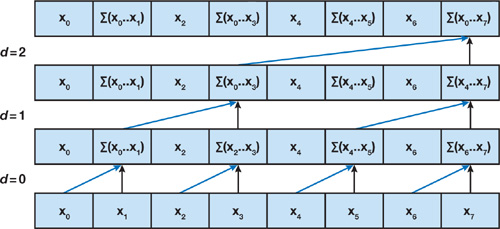
\includegraphics[width=0.5\textwidth]{images/upsweep.jpg}
\caption{Illustration of up-sweep.}
\label{fig:upsweep}
\end{figure}



In the \textbf{down-sweep} phase, the kernel reverses the process, halving the offset at each step and using a simple swapping and summing technique to propagate the sums back through the array in a way that constructs the CDF from the sum tree. This phase starts by setting the last element to zero to ensure the correct initialization for the inclusive scan. \\

\begin{figure}[h]
\centering
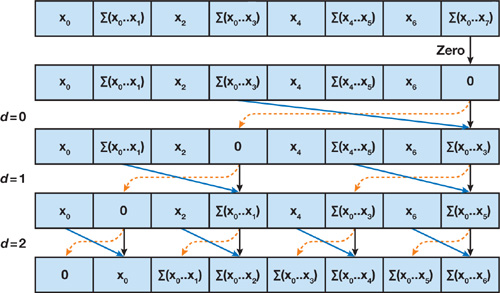
\includegraphics[width=0.5\textwidth]{images/downsweep.jpg}
\caption{Illustration of down-sweep.}
\label{fig:downsweep}
\end{figure}
After completing both phases, each thread writes two elements of the computed CDF back to global memory. 

However the efficient approach still has risk of memory bank conflicts.\\
Memory bank conflicts arise in GPU computing when multiple threads within the same warp access data from the same memory bank of shared memory simultaneously, and at least one of the operations is a write.\\
This would occur after the 2 steps, when each thread writes two values to global memory. \\
Since each memory bank can service only one access per cycle, simultaneous accesses to the same bank cause serialization, leading to increased memory access times and reduced overall performance. These conflicts are a consequence of the parallel architecture of GPUs, where shared memory is divided into multiple banks to allow concurrent accesses by different threads.\\
\pagebreak


\begin{figure}[h]
\centering
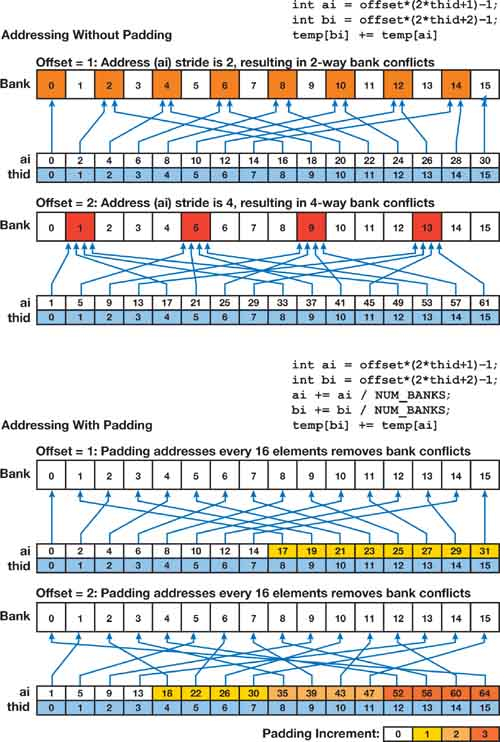
\includegraphics[width=0.5\textwidth]{images/mbk.jpg}
\caption{Illustration of memory bank conflicts.}
\label{fig:mbk}
\end{figure}

\vspace{1cm}

With information given in GPU Gems 3, we can arrive to a strategy for mitigating the conflicts by padding, (intentionally inserting extra space between elements in shared memory) to ensure that consecutive threads access different memory banks. This improves memory access patterns and enhances the efficiency and speed of the kernel shown on next page. 

\pagebreak

\begin{lstlisting}[style=cppstyle]
__global__ void CalculateCDF_we_mbcf(unsigned int* histogram, unsigned int *cdf) {
    __shared__ unsigned int temp[GRAYLEVELS + CONFLICT_FREE_OFFSET(GRAYLEVELS)];

    int tid = threadIdx.x; // 1block 1x128 threads, 128 threads 
    int offset = 1; // distance between elements in array that will be summed

    int ai= 2*tid;
    int bi= tid + (GRAYLEVELS/2);
    int bankOffsetA = CONFLICT_FREE_OFFSET(ai);
    int bankOffsetB = CONFLICT_FREE_OFFSET(bi);
    
    temp[ai + bankOffsetA] = histogram[ai];
    temp[bi + bankOffsetB] = histogram[bi];

    // the sum of values, that each thredad calculates in 1st step

    for (int d = GRAYLEVELS >> 1; d > 0; d >>= 1) {
        __syncthreads();

        if (tid < d) {
            ai = offset*(2*tid+1)-1;
            bi = offset*(2*tid+2)-1;
            temp[bi] += temp[ai];
        }
        offset *= 2;
    }

    if (tid == 0) {
        temp[GRAYLEVELS - 1 + CONFLICT_FREE_OFFSET(GRAYLEVELS - 1)] = 0;
    }
    
    for (int d = 1; d < GRAYLEVELS; d *= 2) {
        offset >>= 1;
        __syncthreads();

        if (tid < d) {
            ai = offset*(2*tid+1)-1;
            bi = offset*(2*tid+2)-1;

            float t = temp[ai];
            temp[ai] = temp[bi];
            temp[bi] += t;
        }
    }
    __syncthreads();
    cdf[ai] = temp[ai + bankOffsetA];
    cdf[bi] = temp[bi + bankOffsetB];
}
\end{lstlisting}

\pagebreak

\subsection{Equalization of the Image}
\vspace{0.3cm}
% Explanation and process of histogram equalization.
The new (equalized) grayscale value is calculated for each pixel like so:\\\\
\begin{equation}
l_{\text{new}} = \frac{\text{cdf}(l) - \text{cdf}_{\text{min}}}{(N \times M) - \text{cdf}_{\text{min}}} \times (L - 1)
\end{equation}


- $l_{new}$ ... being the new value,\\ - $(N \times M)$ ... being the size of an image,\\ - $cdf(l)$ ... being the number of pixels on input image with grayscale value $l$, \\ - $cdf_{min}$ ... being the smallest \textbf{non-zero} value in CDF histogram, 0-s represent no accumulation in the histogram\\ 
- $L$  ... in this case 256, which is the number of gray levels

\vspace{0.3cm}

A kernel for finding the smallest non-zero value in an array, using principle of reduction:\\
\begin{lstlisting}[style=cppstyle]
__global__ void findMinKernel(unsigned int* cdf, unsigned int*d_cdfmin) {
    // Allocate shared memory
	__shared__ unsigned int partial_mins[256];

	// Calculate thread ID
	int tid = threadIdx.x;
    // Load elements into shared memory
    // we are looking for the smallest NON-ZERO value in CDF so we can UINT_MAX all the zeros
    if (tid < 128) {
	    partial_mins[tid] = cdf[tid] == 0 ? UINT_MAX : cdf[tid];
        partial_mins[tid + 128] = cdf[tid + 128] == 0 ? UINT_MAX : cdf[tid + 128];
    }   
    // Start at 1/2 block stride and divide by two each iteration
	for (int s = GRAYLEVELS/2; s > 0; s >>= 1) {
        __syncthreads();
		// Each thread does work unless it is further than the stride
		if (tid < s) {
		    partial_mins[tid] = min(partial_mins[tid], partial_mins[tid + s]); 
	    }
	}
    __syncthreads();
	if (threadIdx.x == 0) {
        *d_cdfmin = partial_mins[0];
	}
}
\end{lstlisting}


\begin{lstlisting}[style=cppstyle]
__device__ unsigned char scale(unsigned int cdf, unsigned int cdfmin, unsigned int imageSize) {
    float scale;
    scale = (float)(cdf - cdfmin) / (float)(imageSize - cdfmin);
    scale = round(scale * (float)(GRAYLEVELS-1));
    return (int)scale;
}
\end{lstlisting}
Device function scale calculates the new value of pixel, according to the equation before.


\pagebreak
 
Kernel bellow builds the new equalized image in parallel, by calling scale function for each pixel with each thread for unique pixel in image. 
BlockSize here is 256 (16*16) and GridSize is calculated the same way as for the histogram calculation kernel.

\begin{lstlisting}[style=cppstyle]
__global__ void EqualizeKernel(unsigned char * image_in, unsigned char * image_out, int width, int height, unsigned int *cdf, unsigned int *cdfmin) {
    unsigned int imageSize = width * height;
    int x = blockIdx.x * blockDim.x + threadIdx.x;
    int y = blockIdx.y * blockDim.y + threadIdx.y;
    
    //Equalize
    if (x < width && y < height){
        image_out[(y*width + x)] = scale(cdf[image_in[y*width + x]], *cdfmin, imageSize);
    }
}
\end{lstlisting}


\section{Implementation testing}
% Explanation and process of histogram equalization.

I have tested my implementation on 7 different images of varying sizes.
I used cudaEvent\_t sturct for timing the execution.
I timed 3 different executions:
- One where all 3 steps are in parallel (Cuda Parallel)
- One where all 3 are sequential (Sequential)
- and One, where I implemented the kernels for sequential execution\\
and ran only 1 thread (Kernel Sequential)

\begin{table}[ht]
\centering
\begin{tabular}{lcccc}
\toprule
\textbf{Image Name} & \textbf{Size of Image $(h \times w)$} & \textbf{Cuda Parallel} & \textbf{ Sequential} & \textbf{Kernel Sequential} \\
\midrule
flower2.jpg & 280 x 180 & 0.1968 ms & 1.2869 ms & 20.8876 ms \\
pa3cio.jpg & 400 x 250 & 0.1918 ms & 2.5469 ms & 52.0048 ms \\
ograja.jpg & 400 x 600 & 0.2159 ms & 6.1029 ms & 230.8772 ms \\
ferari.jpg & 600 x 338 & 0.2082 ms & 5.1372 ms & 197.1191 ms \\
puscava.jpg & 1024 x 683 & 0.3530 ms & 17.7262 ms & 1513.1527 ms \\
flower1.jpg & 1280 x 720 & 0.4385 ms & 23.3550 ms & 2380.4128 ms \\
buca1.jpg & 2560 x 1707 & 1.1806 ms & 110.7117 ms & 49685.0430 ms \\
\bottomrule
\end{tabular}
\caption{Times for parallel and sequential processing.}
\label{tab:processing_times}
\end{table}


\begin{figure}[h]
\centering
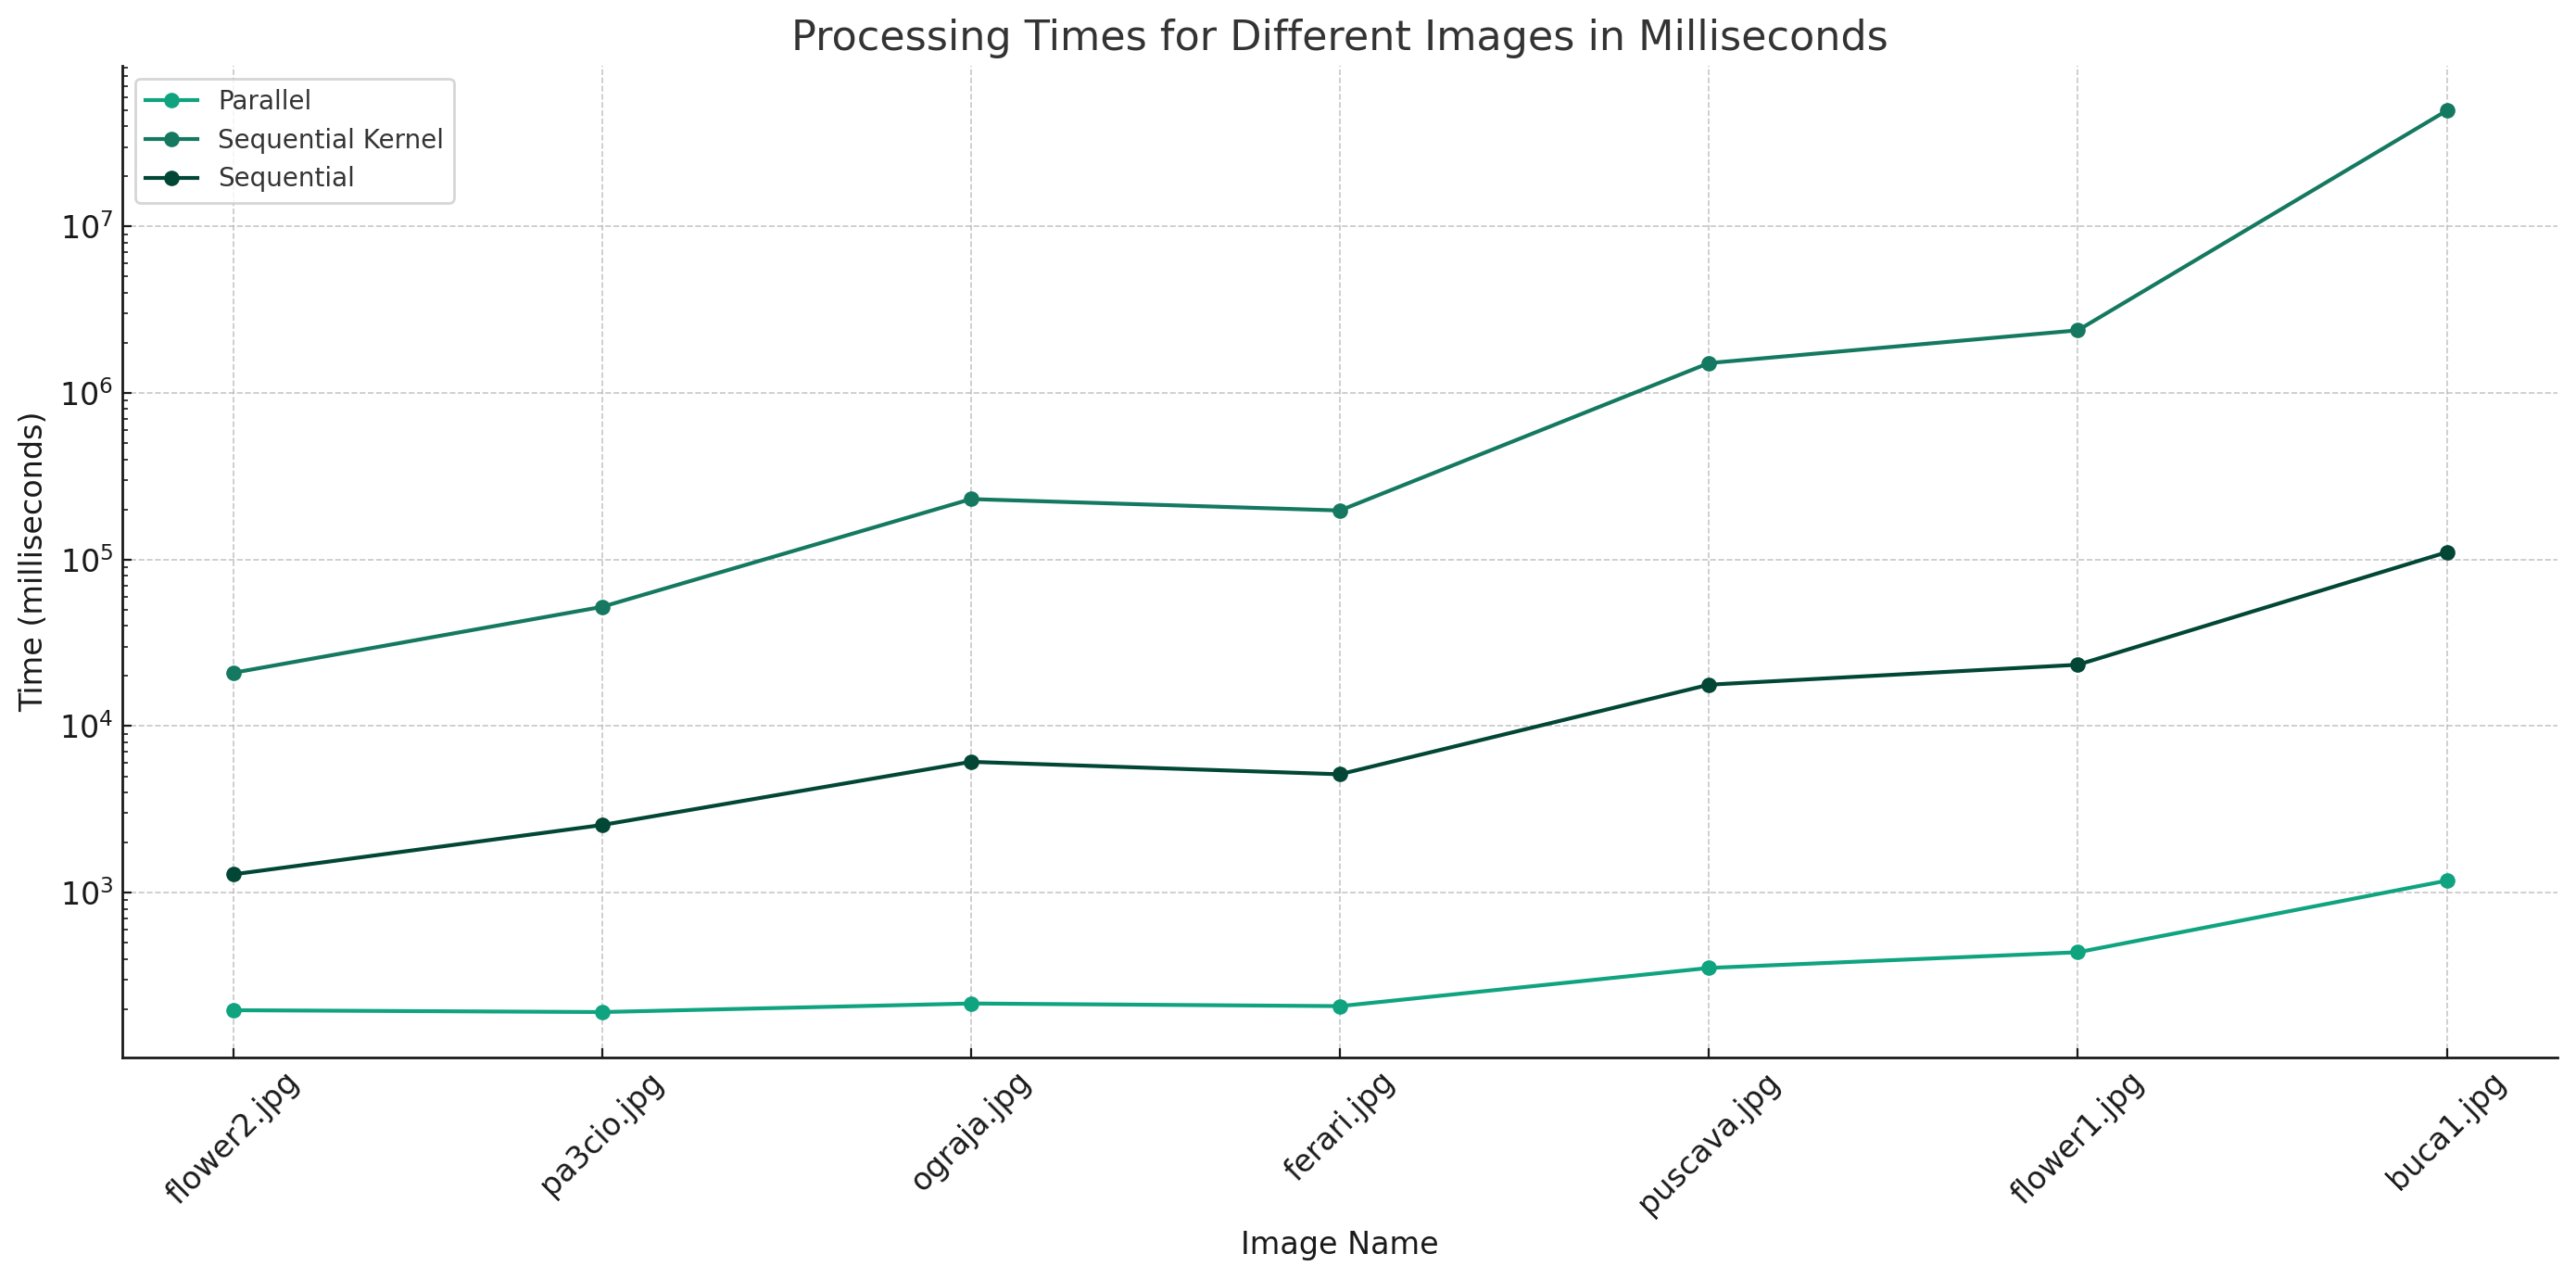
\includegraphics[width=0.9\textwidth]{images/final_time_plot.jpg}
\caption{Graph of times for parallel and sequential processing.}
\label{fig:mbk}
\end{figure}

\pagebreak

\subsection{Image Sample 1}
buca1.jpg

\begin{figure}[ht]
  \centering
  % Subfigure for the original histogram
  \begin{subfigure}[b]{0.4\textwidth}
    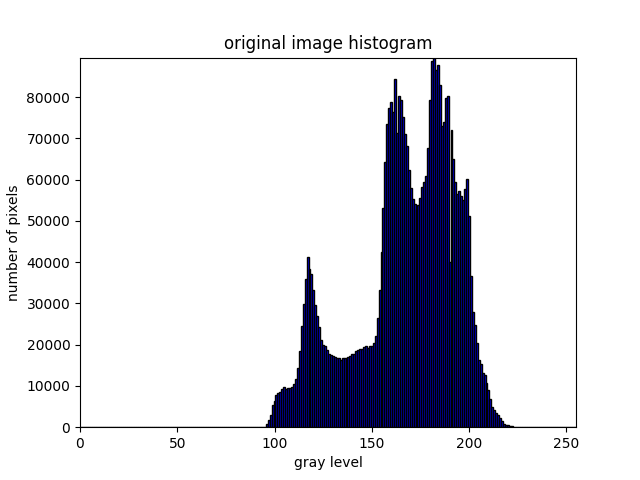
\includegraphics[width=\textwidth]{images/buca-h.png}
    \caption{Original image histogram}
    \label{fig:original-histogram}
  \end{subfigure}
  % Subfigure for the equalized histogram
  \begin{subfigure}[b]{0.4\textwidth}
    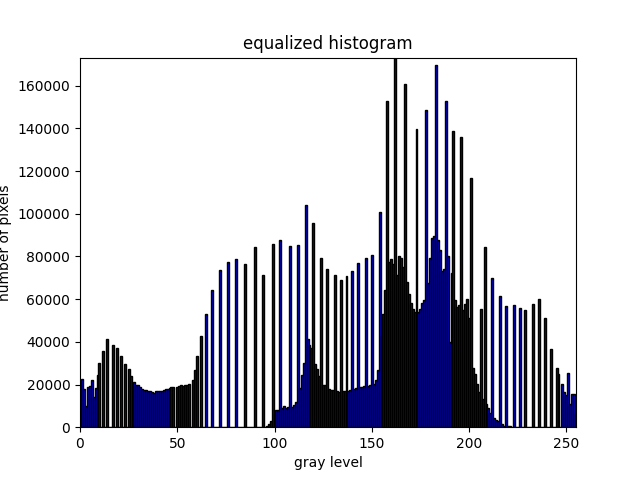
\includegraphics[width=\textwidth]{images/buca-e.png}
    \caption{Equalized histogram}
    \label{fig:equalized-histogram}
  \end{subfigure}
  \caption{Comparison of original and equalized histograms, for image buca1.jpg}
\end{figure}

\begin{figure}[ht]
  \centering
  % Subfigure for the original histogram
  \begin{subfigure}[c]{0.4\textwidth}
    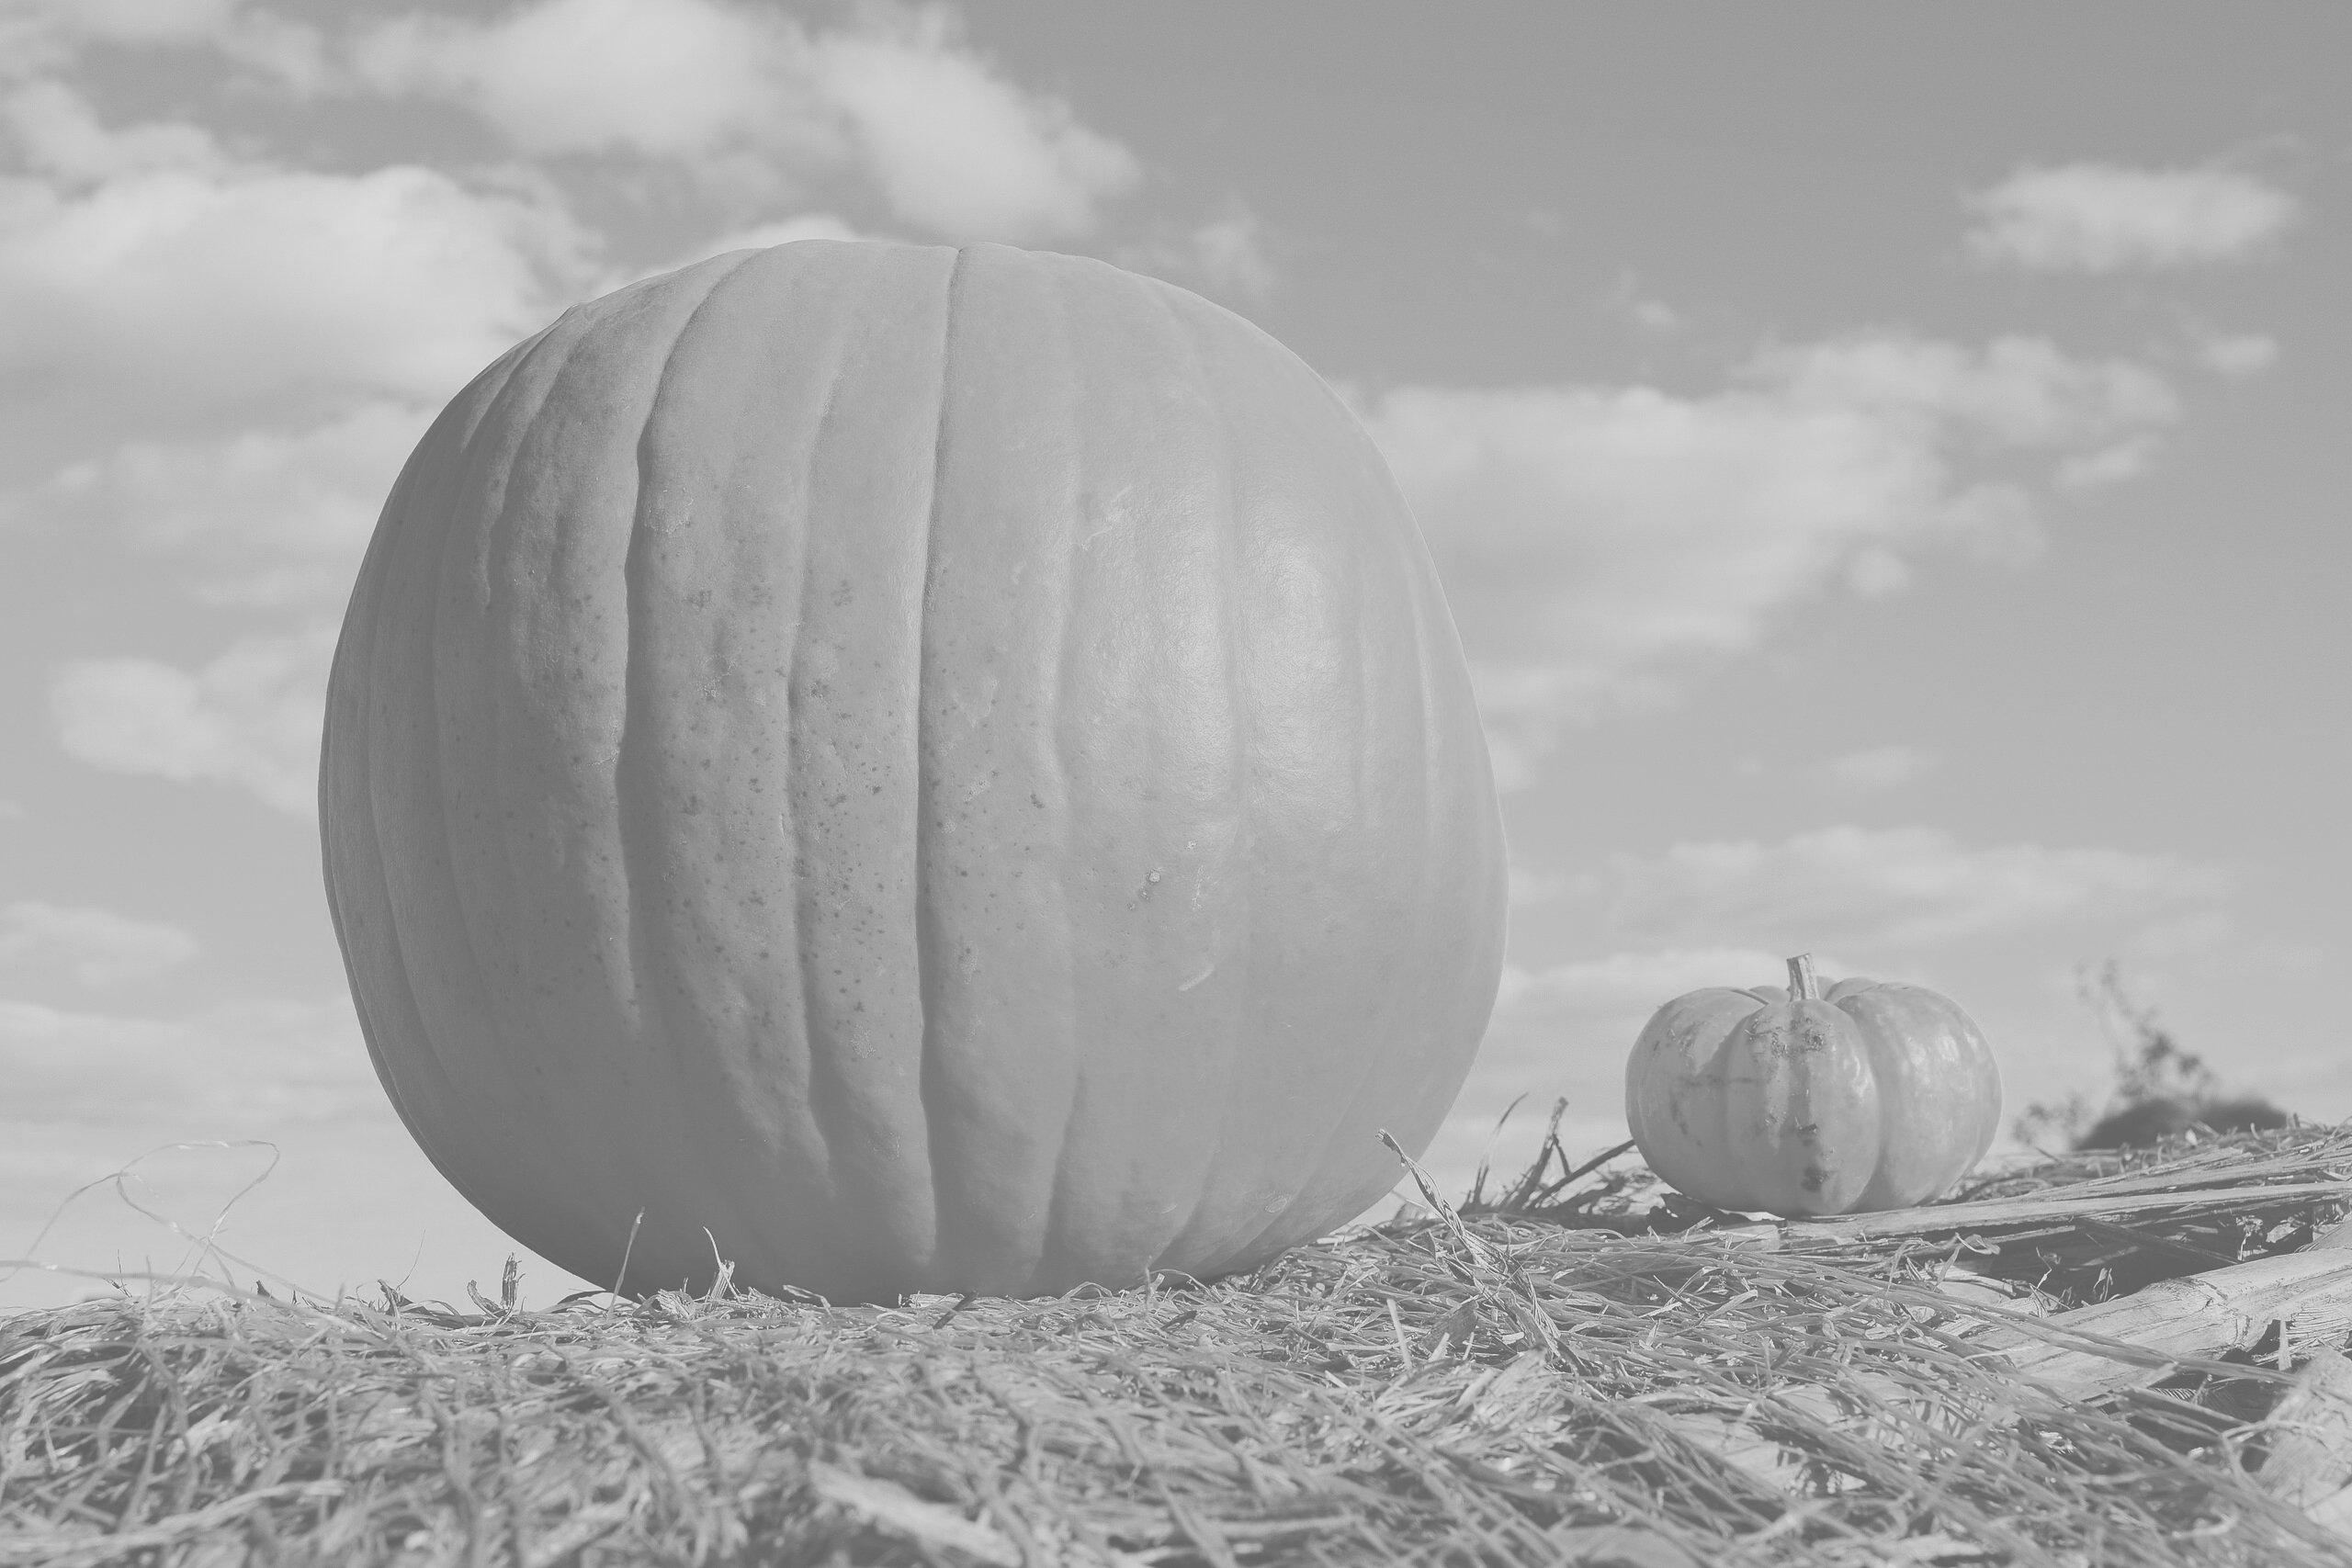
\includegraphics[width=\textwidth]{images/buca1.jpg}
    \caption{Oringinal image}
    \label{fig:original-histogram}
  \end{subfigure}
  % Subfigure for the equalized histogram
  \begin{subfigure}[d]{0.4\textwidth}
    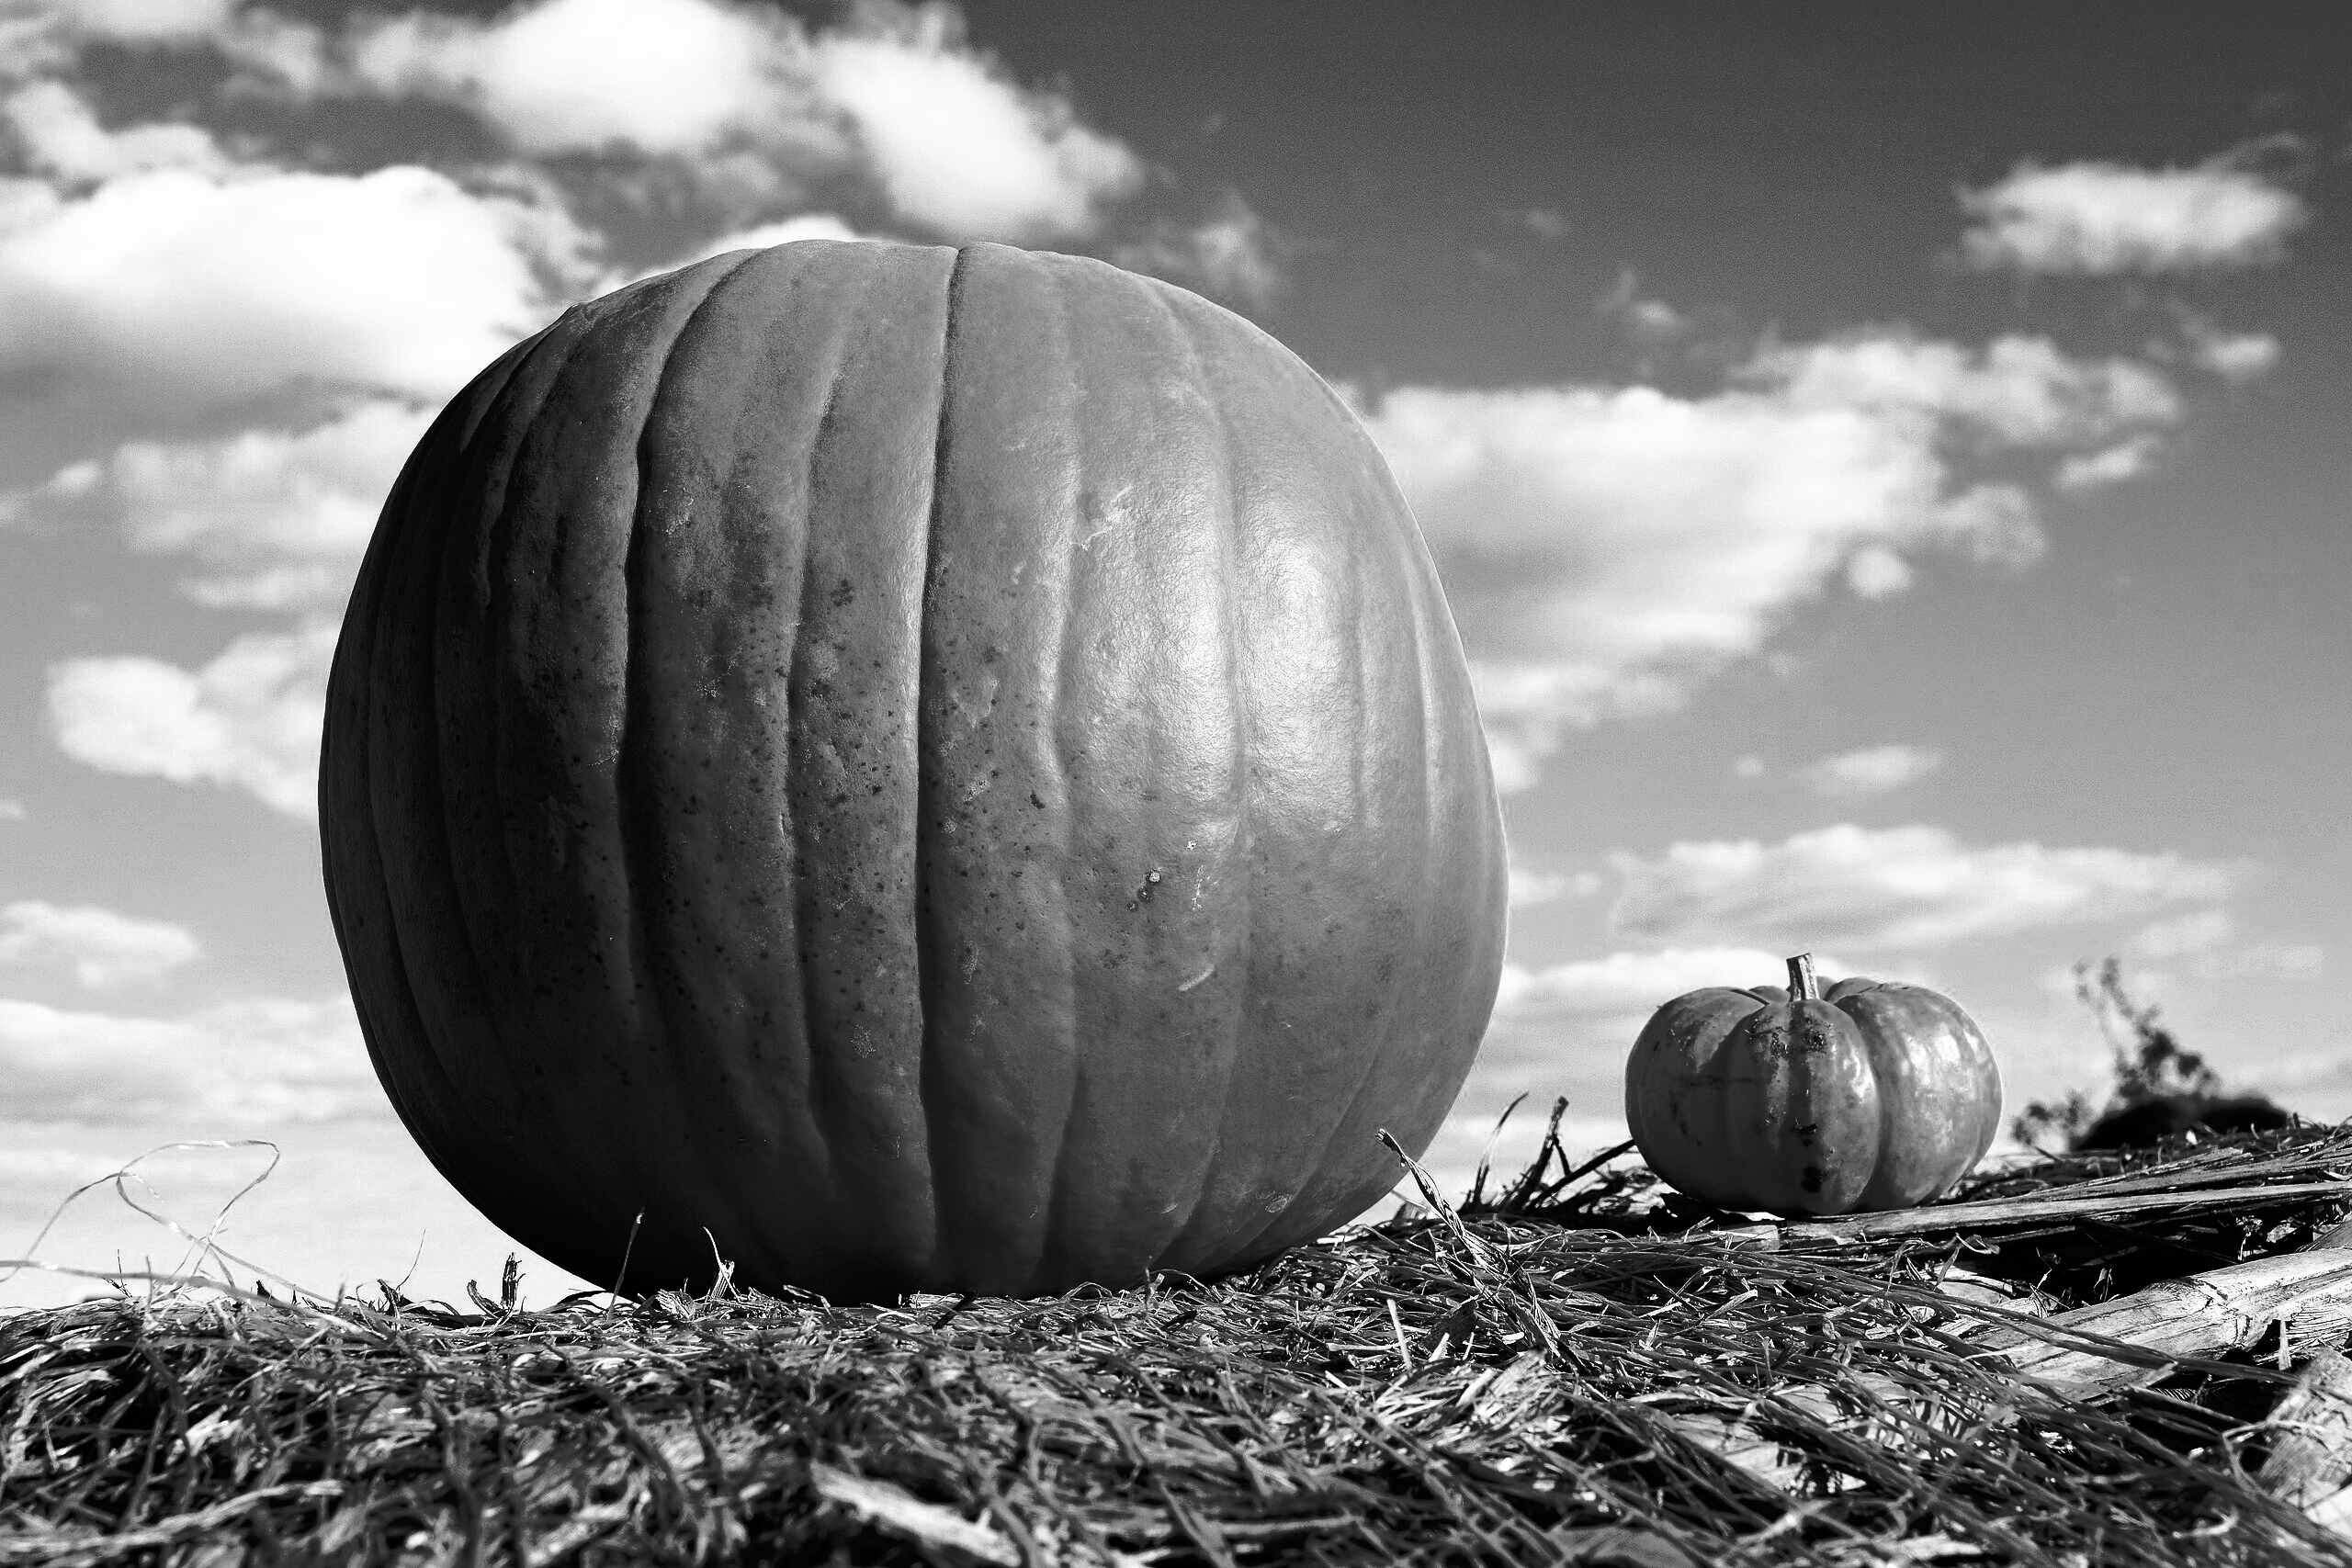
\includegraphics[width=\textwidth]{images/buca1_out.jpg}
    \caption{Equalized image}
    \label{fig:equalized-histogram}
  \end{subfigure}
  \caption{Comparison of original and equalized histograms, for image buca1.jpg}
\end{figure}

\pagebreak

\subsection{Image Sample 2}
pa3cio.jpg\\

\begin{figure}[!ht]
  \centering
  % Subfigure for the original histogram
  \begin{subfigure}{0.4\textwidth}
    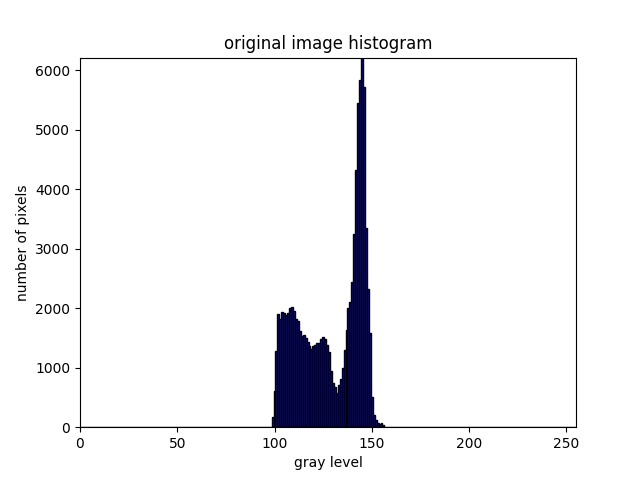
\includegraphics[width=\textwidth]{images/pa3cio-h.png}
    \caption{Original image histogram}
    \label{fig:pa3cio-original-histogram}
  \end{subfigure}
  % Subfigure for the equalized histogram
  \begin{subfigure}{0.4\textwidth}
    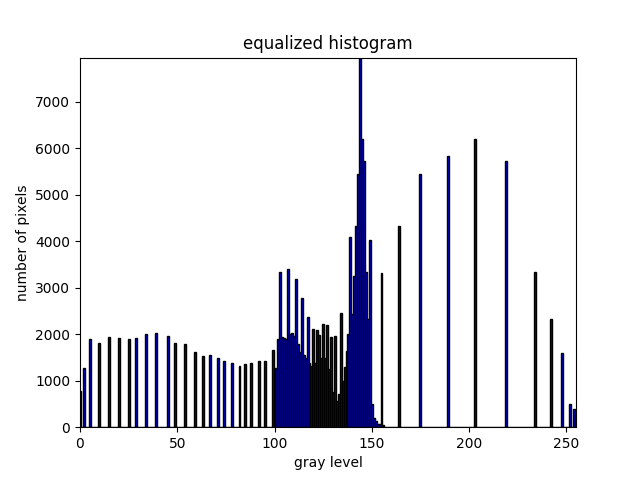
\includegraphics[width=\textwidth]{images/pa3cio-e.png}
    \caption{Equalized histogram}
    \label{fig:pa3cio-equalized-histogram}
  \end{subfigure}
  \caption{Comparison of original and equalized histograms, for image pa3cio.jpg}
\end{figure}

\begin{figure}[!ht]
  \centering
  % Subfigure for the original image
  \begin{subfigure}{0.4\textwidth}
    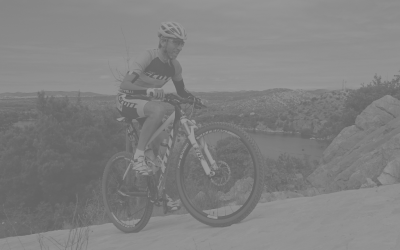
\includegraphics[width=\textwidth]{images/pat3cio-neq.jpg}
    \caption{Original image}
    \label{fig:pa3cio-original}
  \end{subfigure}
  % Subfigure for the equalized image
  \begin{subfigure}{0.4\textwidth}
    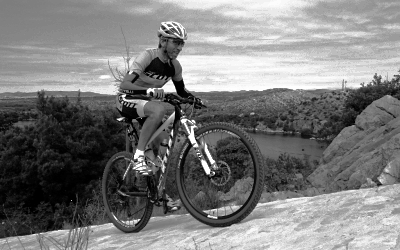
\includegraphics[width=\textwidth]{images/pa3cio-neq_out.jpg}
    \caption{Equalized image}
    \label{fig:pa3cio-equalized}
  \end{subfigure}
  \caption{Comparison of original and equalized images, for image pa3cio.jpg}
\end{figure}

\pagebreak

\subsection{Image Sample 3}
flower1.jpg\\

\begin{figure}[!ht]
  \centering
  % Subfigure for the original histogram
  \begin{subfigure}[b]{0.4\textwidth}
    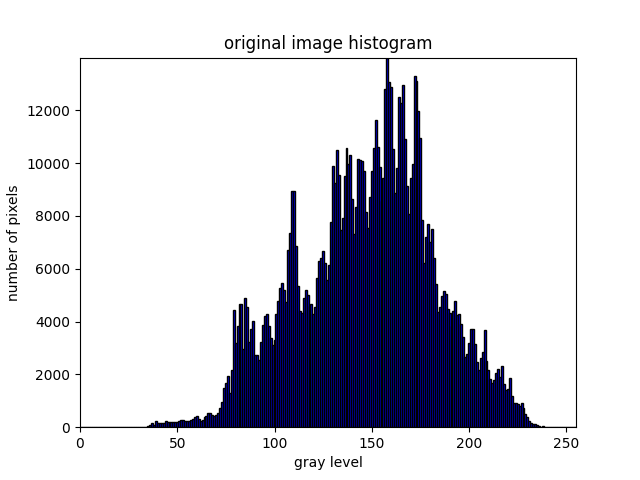
\includegraphics[width=\textwidth]{images/flower1-h.png}
    \caption{Original image histogram}
    \label{fig:original-histogram}
  \end{subfigure}
  % Subfigure for the equalized histogram
  \begin{subfigure}[b]{0.4\textwidth}
    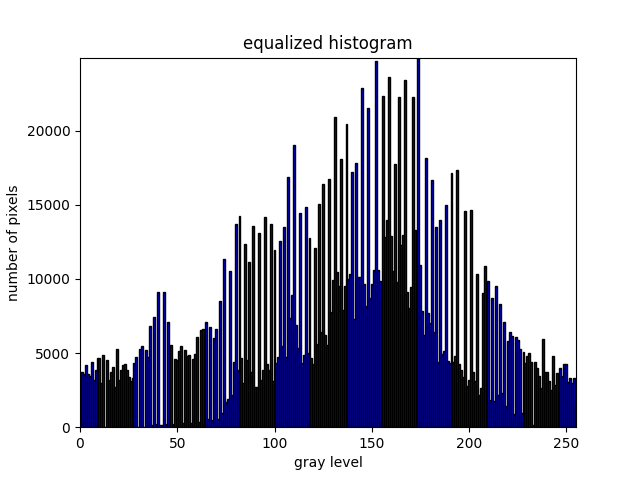
\includegraphics[width=\textwidth]{images/flower1-e.png}
    \caption{Equalized histogram}
    \label{fig:equalized-histogram}
  \end{subfigure}
  \caption{Comparison of original and equalized histograms, for image buca1.jpg}
\end{figure}

\begin{figure}[ht]
  \centering
  % Subfigure for the original histogram
  \begin{subfigure}[c]{0.4\textwidth}
    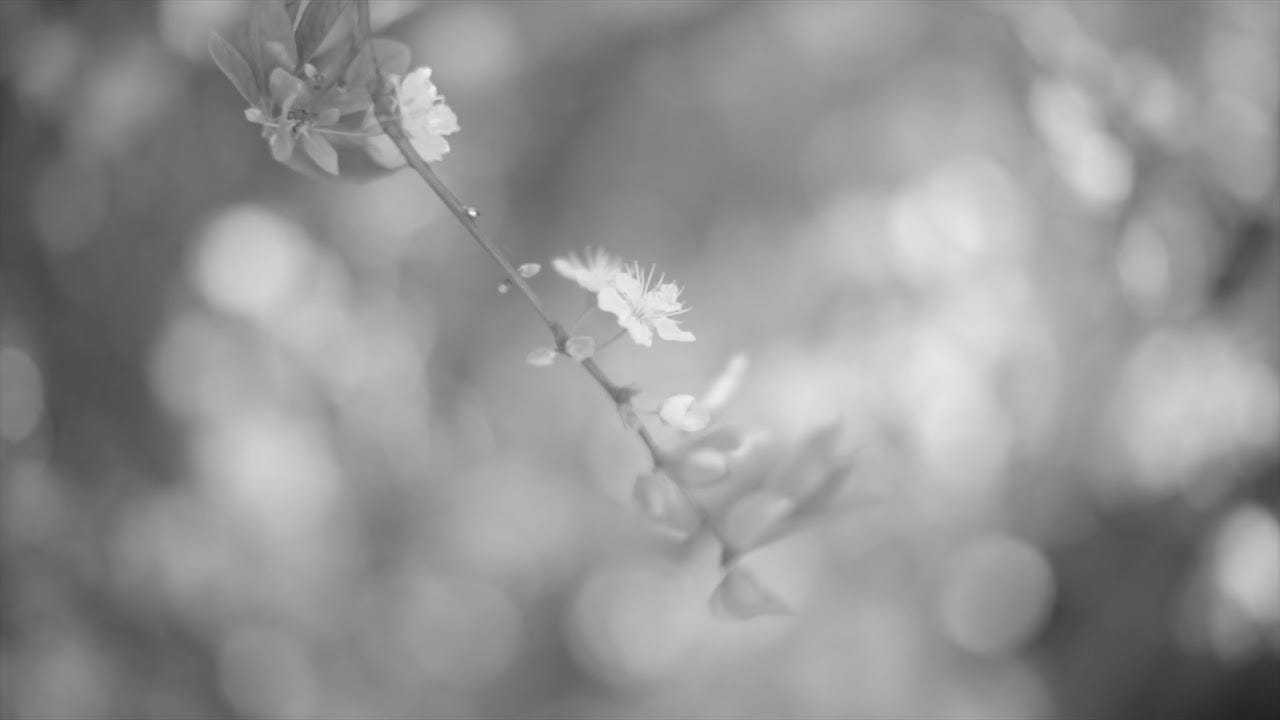
\includegraphics[width=\textwidth]{images/flower1-neq.jpg}
    \caption{Oringinal image}
    \label{fig:original-histogram}
  \end{subfigure}
  % Subfigure for the equalized histogram
  \begin{subfigure}[d]{0.4\textwidth}
    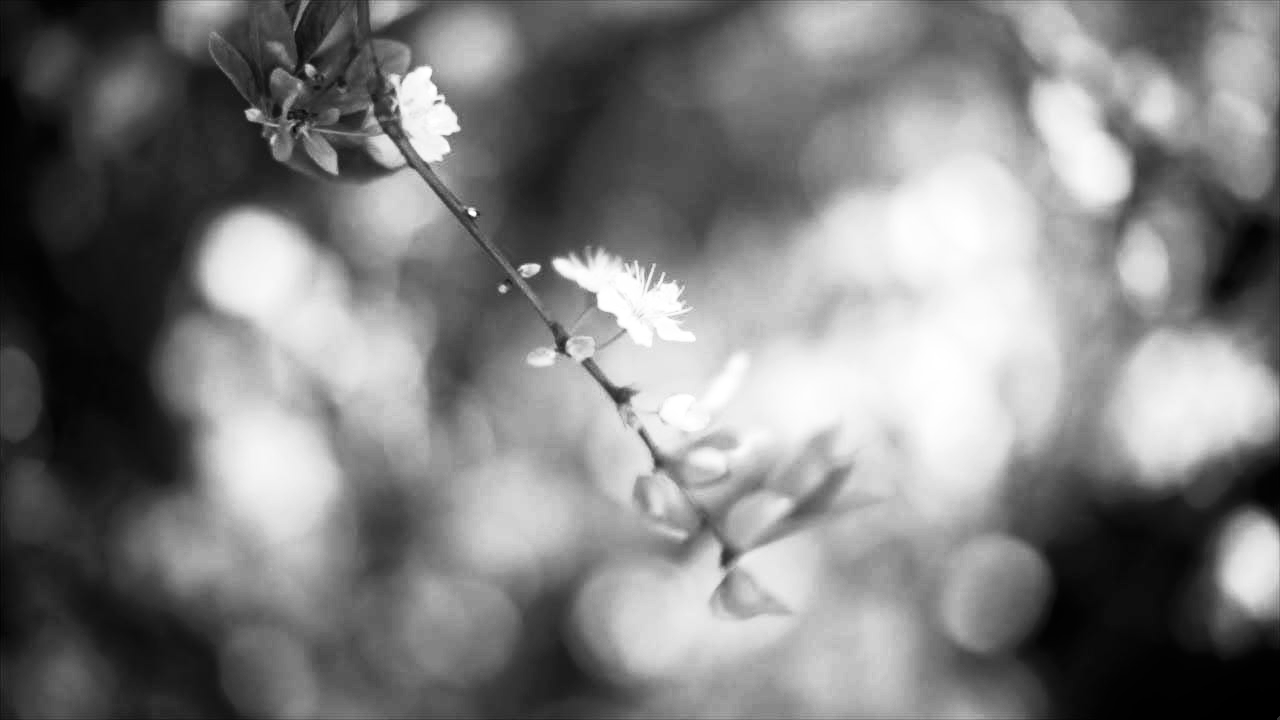
\includegraphics[width=\textwidth]{images/flower1-neq_out.jpg}
    \caption{Equalized image}
    \label{fig:equalized-histogram}
  \end{subfigure}
  \caption{Comparison of original and equalized histograms, for image buca1.jpg}
\end{figure}

\pagebreak

\section{Results and Conclusion}
\label{sec:Introduction}

In conclusion of this report, the comparative analysis between parallel and sequential processing methodologies for the task of gray-scale image histogram equalization has shown a substantial difference between each. The results unambiguously support the hypothesis that parallel computing, particularly when executed on Graphics Processing Units (GPUs), is superior in performance relative to its sequential counterpart running on Central Processing Units (CPUs).

Throughout the range of sample sizes subjected to testing, it has been consistently observed that the parallel implementation outpaces sequential processing. The distinction in performance, while noticeable even at smaller scales, becomes stark as the dimensions of the image increase. This trend can be attributed to the intrinsic nature of parallel computing, which, unlike sequential processing, can simultaneously handle multiple data points. GPUs, with their multitude of cores designed for concurrent operations, are particularly adept at managing large sets of pixel data inherent in high-resolution images. \\
Parallel processing is not always the optimal approach due to several limiting factors, most notably described by Amdahl's Law. Amdahl's Law provides a theoretical maximum improvement in performance using parallel processing and highlights the importance of sequential execution time in the overall computation. The law can be expressed by the formula:


\begin{equation}
S_{\text{latency}}(s) = \frac{1}{(1 - p) + \frac{p}{s}}
\end{equation}

where
\begin{itemize}
\item \( S_{\text{latency}} \) is the theoretical speedup of the execution of the whole task,
\item \( s \) is the speedup of the part of the task that benefits from improved system resources,
\item \( p \) is the proportion of the task that can be parallelized (i.e., the proportion of execution time that the part benefiting from improved resources originally occupied).
\end{itemize}

\vspace{1cm}

According to Amdahl's Law, the speedup of a program using multiple processors in parallel computing is limited by the time needed for the sequential fraction of the program. For instance, if only 50\% of a program can be parallelized, the maximum speedup using parallel computing would be 2x, no matter how many processors are used. This implies that there is a point of diminishing returns where adding more processing power yields minimal improvements. This is because the non-parallelizable part of the program (the sequential component) becomes a bottleneck.


\pagebreak
\section{References}
GPU Gems 3 web article \citep{GPU_Gems_3}.
Fri ucilnica \citep{Fri_ucilnica}

\pagebreak




% BIBLIOGRAPHY %%%%%%%%%%%%%%%%%%%%%%%%%%%%%%%%%%%%%%%%%%%%%%%%%%%%%%%%%%%%%%%%%%%%%%%%%%%%%%%%%%%% 

% Use Leeds Harvard referencing template
\bibliographystyle{unsrt}
% Add here the bib file with your references
\bibliography{references}

\clearpage
\end{document}

